\documentclass[UTF8]{article}
\usepackage{ctex}
\usepackage{ulem}
\usepackage{amssymb}
\usepackage{amsmath}
\usepackage{graphicx}
\newtheorem{thm}{定义}[section]
\newtheorem{notation}[thm]{记号}
\newtheorem{lemma}[thm]{引理}

\makeatletter
\newcommand{\rmnum}[1]{\romannumeral #1}
\newcommand{\Rmnum}[1]{\expandafter\@slowromancap\romannumeral #1@}
\makeatother

\title{依赖于项的类型\\[2ex]\begin{large}读书笔记\end{large}}
\author{许博}
\date{}

\begin{document}
\maketitle
	\section{疑问}
		在PAT-解释的时候,对于任意蕴含式,是否只要蕴含式中所有的命题为真,都可以构建对应类型的项,并且表示蕴含式为真?且当存在某一命题为假时,是否无法构建项,此时能否判定蕴含式为假?如果是的话,前件为假的时候蕴含式为真的情况如何处理?如果将蕴含式看作一个命题的话,没有对应类型的项的时候判断命题为假是不是不正确,或者是否不能进行这样的判断?而是只能判断蕴含式在前件为真时是否为重言式?并且在无法判断是否为重言式的时候也不能得到其为假的结果?

	\section{遗失的扩展}
		之前已经引入了依赖于项的项,依赖于类型的项以及依赖于类型的类型,本章将在$\lambda{\rightarrow}$的基础上引入依赖于项的类型,记为$\lambda{\rm P}$。
		
		一个依赖于一个项的类型具有如下一般形式:
		
		\begin{center}
			$\lambda x:A.M$,
		\end{center}
	
		其中$M$是一个类型,$x$是一个项变量(所以$A$必须是一个类型)。抽象$\lambda x:A.M$依赖于项$x$。
		
		与 Remark 4.1.2 相对应,一个依赖于项的类型事实上是一个类型作为值的函数或者类型构造子。
		
		将$M$特化成集合或命题,观察依赖于项的类型的用处:
		
		(1) 令$S_n$是一个对于任一$n:nat$的集合,将集合看作是类型。$\lambda n:nat.S_n$是一个函数映射项$n$到集合$S_n$,所谓的集合作为值的函数。其它的术语是,这个抽象是一个类型族(a family of types)或者一个索引类型(被$n:nat$索引)。显而易见的是,$\lambda n:nat.S_n$的类型是$nat\rightarrow*$。
		
		(2) 令$P_n$是一个对于任一$n:nat$的命题,将命题看作类型(也即之前提到过的PAT-解释)。这样的函数在逻辑中表示谓词。比如,令$P_n$是命题“$n$是一个质数”。抽象$\lambda n:nat.P_n$就是一个逻辑谓词表示“是质数”(对于自然数来说)。
		
		应用:\\—\ $(\lambda n:nat.S_n)3$,\\—\ $(\lambda n:nat.P_n)3$。
		
		两个表达式都表示依赖于项(即3)的类型。
		
	\section{$\lambda{\rm P}$的推导规则}
		$\lambda{\rm P}$的所有规则:

		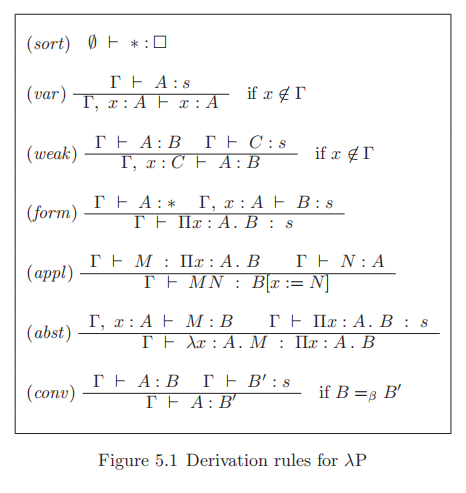
\includegraphics[width=0.93\linewidth]{"../imgs/5-1.png"}
		
		$\lambda{\rm P}$的推导规则与$\lambda{\uline{\omega}}$的规则十分相似,其中的(sort), (var), (weak) 以及 (conv) 规则都相同。
		
		与$\lambda{\uline{\omega}}$的主要不同之处是:
		
		(i) $\rightarrow$-类型的升级。不再使用$A\rightarrow B$而是$\Pi x:A.B$,因为变量$x$可能作为自由变量出现在$B$中。如$\lambda x:nat. \lambda s:(\lambda n:nat.S_n)x. s$的类型是$\Pi x:nat.\Pi s:S_x.S_x$。
		
		(ii) 输入类型的降级。$\lambda{\rm P}$中,对于类型$\Pi x:A.B$,有$x$是一个项,所以$A$只能具有类型$*$。
		
		需要注意的是,在(form)规则中有:
		
		(1) $s = *$,则$A:*,B:*$且$\Pi x:A.B:*$,
		
		(2) $s = \square$,则$A:*,B:\square$且$\Pi x:A.B:\square$。
		
		对于$\Pi x:A.B$,如果可以确定$x$不(作为自由变量)出现在$B$中,则可以非正式地写为$A\rightarrow B$。
		
	\section{$\lambda{\rm P}$中的推导实例}
		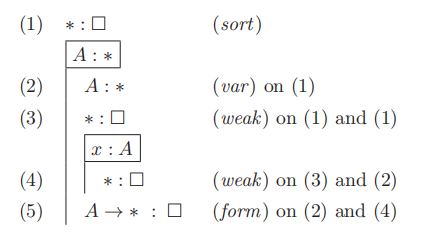
\includegraphics[width=0.93\linewidth]{"../imgs/5-2.png"}
		
		需要注意的是,$A\rightarrow*$作为依赖于项的类型的类型,是一个依赖于一个项的种类(kind),而$P:A\rightarrow*$则是一个依赖于一个项的类型。
		
		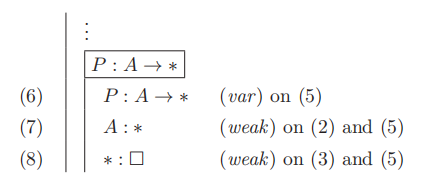
\includegraphics[width=0.93\linewidth]{"../imgs/5-3.png"}
		
		将$P$应用于$x$可以得到类型$Px$:
		
		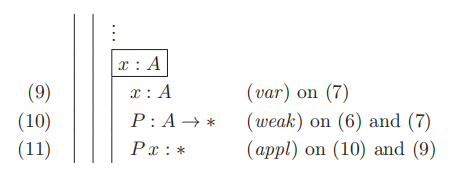
\includegraphics[width=0.93\linewidth]{"../imgs/5-4.png"}
		
		第(11)行允许我们构建一个真正的依赖类型:
		
		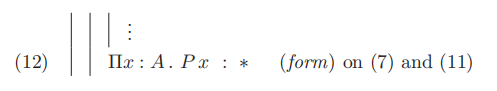
\includegraphics[width=0.93\linewidth]{"../imgs/5-5.png"}
		
		然后我们可以推导出类型$Px\rightarrow Px$,之后再构建另一个$\Pi$-类型,即$\Pi x:A.Px\rightarrow Px$:
		
		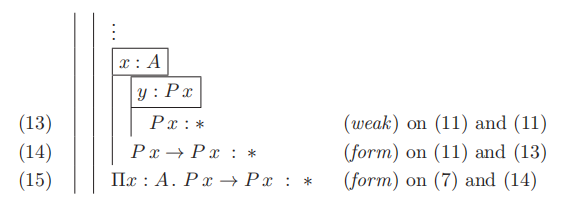
\includegraphics[width=0.93\linewidth]{"../imgs/5-6.png"}
		
		最后,可以推导出一个类型是$\Pi x:A.Px\rightarrow Px$的项:
		
		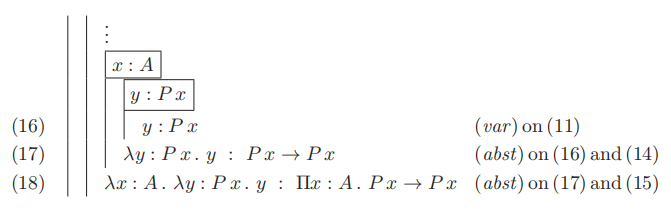
\includegraphics[width=0.93\linewidth]{"../imgs/5-7.png"}
		
		这个推导也可以看作是在 2.6 节中提到的三个问题的一个解决方案:良好的类型定义,类型检查以及项的查找。
		
		简化一些过程的简短推导为:
		
		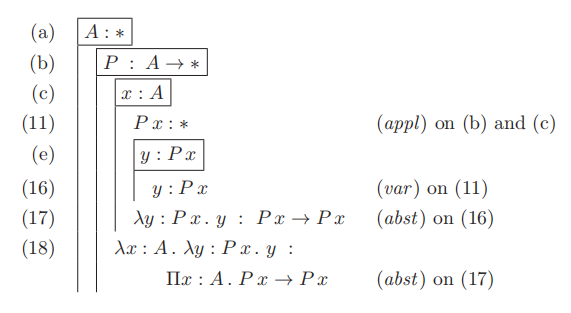
\includegraphics[width=0.93\linewidth]{"../imgs/5-8.png"}
		
	\section{$\lambda{\rm P}$中的最小谓词逻辑}
		在$\lambda{\rm P}$中可以编写一种非常简单的逻辑形式,叫做最小谓词逻辑(minimal predicate logic),只包含了蕴含以及全称量词作为逻辑运算。这个谓词逻辑中的基础实体是前提,集合以及集合上的谓词。
		
		PAT-解释(propositions-as-types/proofs-as-terms interpretation):\\
		—\ 如果$b:B$,$B$被解释为命题,则将$b$解释为$B$的一个证明。这样的项在类型理论中被叫做一个证明对象(proof object)。\\
		—\ 另一方面,如果不存在$b$使得$b:B$,则不存在命题$B$的证明,所以$B$一定为假。
		
		现在给出最小谓词逻辑的基础实体的编写以及在恰当的情况下应用完整的PAT-解释:
		
		\noindent
		\textit{\Rmnum{1}. 集合}\\
		将一个集合$S$作为一个类型,所以$S:*$。集合中的元素是项。所以如果$a$是集合$S$中的一个项,则$a:S$。如果$S$是空的集合,则不存在可推导的项$a$使得$a:S$。
		
		例:$nat:*, nat\rightarrow nat:*; 3:nat, \lambda n:nat.n:nat\rightarrow nat$。\\
		
		\noindent
		\textit{\Rmnum{2}. 命题}\\
		将命题作为类型,所以如果$A$是一个命题,则$A:*$。根据PAT-解释,如果$A$是真命题,则存在$p:A$,$p$是$A$的一个证明。如果不存在$A$的证明,即$p:A$,则$A$为假。\\
		
		\noindent
		\textit{\Rmnum{3}. 谓词}\\
		一个谓词$P$是一个从一个集合$S$到所有命题集合的一个函数。所以$P:S\rightarrow*$。如果$P$是一个在$S$上的任意的谓词,则对每个$a:S$,都有$Pa:*$。所有的$Pa$都是命题,因此:
		
		(1) 如果存在$t:Pa$,则这个命题在$a$上成立。
		
		(2) 如果不存在$t:Pa$,则这个命题在$a$上不成立。\\
		
		\noindent
		\textit{\Rmnum{4}. 蕴含式}\\
		在类型理论中,将蕴含式$A\Rightarrow B$写作函数类型$A\rightarrow B$。也即如果存在类型为$A\rightarrow B$的函数,即可证明对应的蕴含式为真:\\
		
		$A\Rightarrow B$为真;
		
		如果$A$为真,则$B$也为真;
		
		如果$A$有成员,则$B$也有成员;
		
		存在一个函数映射$A$的成员到$B$的成员;
		
		存在一个函数$f:A\rightarrow B$;
		
		$A\rightarrow$有成员。\\
		
		\noindent
		\textit{\Rmnum{5}. 全称量词}\\
		考虑全称量词$\forall_{x\in S}(P(x))$,即在集合$S$上依赖于$x$的谓词$P$。可以进行如下PAT-解释:\\
		
		$\forall_{x\in S}(P(x))$为真;
		
		对于集合$S$中的每个$x$,命题$P(x)$为真;
		
		对于$S$中的每个$x$,类型$Px$有成员;
		
		存在一个函数映射$S$中的每个$x$到$Px$的一个成员,即具有类型$\Pi x:S.Px$的函数;
	
		存在一个函数$f:\Pi x:S.Px$;
		
		$\Pi x:S.Px$具有成员。\\
		
		与蕴含式类似,我们将全称量词解释为$\Pi$-类型。
		
		需要注意的是,与前文提到的$P:A\rightarrow*$一样,$\Pi x:S.Px$也是一个依赖于项$x$的类型(构造子),尽管两者所处的位置可能不同。
		
		给出$\forall$的消解(elimination)和导入(introduction)规则:
		
		($\forall-elim$)\ $\cfrac{\forall_{x\in S}(P(x))\ \ \ \ N\in S}{P(N)}$
		
		这个规则的含义是:如果对于$S$中的每一个$x$谓词$P$都成立,则对于给定的$S$中的$N$,谓词$P$成立。
		
		($\forall-intro$)\ $\cfrac{let\ x\in S\ \ \ P(x)}{\forall_{x\in S}(P(x))}$
		
		也即,如果对于任意的$x\in S$,谓词$P$都成立,则对于所有的$x\in S$,谓词$P$都成立。
		
		需要注意的是,最小谓词逻辑(或$\lambda{\rm P}$)中,没有否定,合取,析取以及存在量词。目前最小谓词逻辑和$\lambda{\rm P}$相对应的结构如下图:
		
		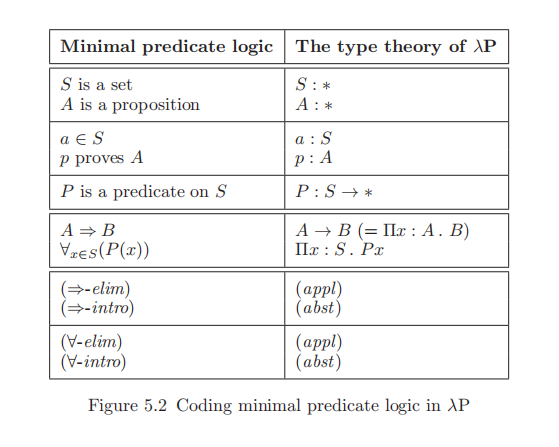
\includegraphics[width=0.93\linewidth]{"../imgs/5-9.png"}
		
\end{document}
